\documentclass{article}
\usepackage[utf8x]{inputenc}
\usepackage{times}
\usepackage[intlimits,sumlimits]{amsmath}
\usepackage{amssymb}
\usepackage{graphicx}
\usepackage{hyperref}
% listings begin
\usepackage{color}
\usepackage{xcolor}
\usepackage{listings}
\usepackage{caption}
\DeclareCaptionFont{white}{\color{white}}
\DeclareCaptionFormat{listing}{\colorbox{gray}{\parbox{\textwidth}{#1#2#3}}}
\captionsetup[lstlisting]{format=listing,labelfont=white,textfont=white}
% listings end
%opening
\author{Milán Unicsovics}
\title{Project Laboratory 2}
\date{\today}

% Prevent too long lines
\sloppy
\begin{document}
%%%%%%%%%%%%%%%%%%%Titlepage%%%%%%%%%%%%%%%%%%%%%%
\begin{titlepage}

\begin{figure}[htp]
\centering
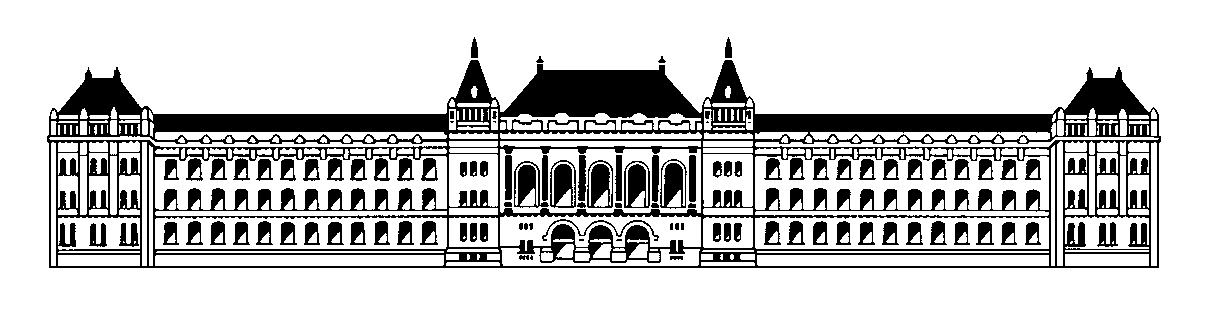
\includegraphics[scale=0.3]{img/bme.png}
\begin{center}
Budapest University of Technology and Economics\\
Department of Measurement and Information Systems
\end{center}
\end{figure}

\vspace{3cm}
\begin{center}
\textsc{\LARGE \textbf{Test generation based on state machine models}}
\vspace{0.5cm}\\
Project Laboratory 2 final report\\
2014/15. I. semester

\vspace{3cm}
\textsc{\large \textbf{Milán György Unicsovics (M9GNTV)}}
\vspace{0.5cm}\\
I. year, computer engineering student\\
MSc Specialization in Dependable System Design

\vspace*{\fill}

Consultant:\\
Dr. Zoltán Micskei assistant professor, MIT\\[0.3cm]

\end{center}

\end{titlepage}
%
\tableofcontents
\newpage
%%%%%%%%%%%%%%%%%%%Text%%%%%%%%%%%%%%%%%%%%%%

\section{Introduction}
\label{sec:intro}

The main goal of software testing is fault detection, where we compare the software's intended and actual behaviour to make sure there are not any difference between those, regarding the requirements.

These methods are usually very time and resource consuming activities. The process is often undocumented, unrepeatable and unstructured, that's why creating tests limited by the ingenuity of the single developer. Furthermore the traditional test cases are static and hard to update, but the software under test is dynamically evolving. One other problem of the handcrafted test is, that they suffer from "pesticide paradox". The test are getting less effective during the testing process, because the tester writes them with the same method for mostly solved problems.

Model-based testing substitutes the traditional ad-hoc software testing methods which relies on behaviour models that describe the intended behaviour of the system and its environment. Set of test cases are generated automatically from the models and then executed on the tested software.

My research aims to prepare to create a new automated testing framework for software based on state machine models. Before that related works and similar solutions have to be examined. The result of the research later can be used to design and develop a software which fills the need of a fully automated model based testing framework.\newline

Previous year I investigated the model based testing process. I became familiar with the terminology and taxonomy of the model based testing process. After that available testing tools have been analysed concentrating on their test case selection criteria. I examined two lightweight model based testing tools (GraphWalker \cite{graphwalker} and PyModel \cite{pymodel}) to see some comprehensible, real world examples of industrial tools. Based on the experiences I wanted to implement a prototype where I can try out some of the learned techniques. To implement a prototype of a testing framework I studied graph based algorithm. I decided to implement the framework driven by the Chinese Postman Problem. This algorithm can generate use cases effectively on resettable softwares, which can step back to their start state. The implemented software could make a single test case for a given software, that contains all method call in the software.

In this year I concertised my long term goal on my thesis. This will be test generation from Papyrus \cite{papyrus} UML state charts. The planned framework will consists Eclipse technologies as Papyrus model editor, my test generator plugin for Papyrus and the Eclipse IDE for writing the software's code. With this framework the user will be able to generate test cases for a given software. The process is the following:

\begin{enumerate}
	\item The user creates a model in Eclipse Papyrus, that acts as the model of software under test (SUT). This model can be for example an UML like state chart model.
	\item The model of the Papyrus state chart will be transformed with model transformation to an intermediate model. This is necessary because UML state charts are on a higher level, and the test case generation algorithms can not be apply directly on them. These algorithms are usually defined on lower level models, for example on finite state machines.
	\item The selected test case generation algorithms can be executed on the intermediate model. These are the abstract test cases.
	\item The abstract test cases have to be transformed into concrete test cases, which can be executed on the software.
\end{enumerate}

After defining the test generation process, I specified my goals in this semester. The most important thing is to find a flexible intermediate language, that's abstraction level is somewhere between the UML state charts and finite state machines. The second task is to find a test generation algorithm that can be executed on the given intermediate language and fulfils the selected criteria. The search can be accomplished by studying related works and available model based testing tools.

% section intro (end)

\section{Test case generation}
\label{sec:testcasegen}

Investigating test case generation algorithms is important, because it has a strong impact on the effectiveness of software testing \cite{testcasegen} \cite{mbttestcasegeneration}. That's why this topic is under activate research and resulted different approaches. The available method should be studied, because the efficiency can be improved by combining these methods.

\subsection{Symbolic execution}
\label{sub:symbolicexecution}

Symbolic execution is a program analysis technique that analyses a program’s code to automatically generate test cases from it. It belongs to white box testing, because the inner structure of the SUT is known during the test.

Symbolic execution uses symbolic values, instead of concrete values, as program inputs. During the symbolic execution the state of the program is represented with \textit{symbolic values} of program variables at that point, a \textit{path constraint} created by symbolic values, and a \textit{program counter}. The path constraint is a Boolean formula, that has to be satisfied to reach that point on the path. At each branch point the path constraint is updated with constraints of the inputs. If the path constraint becomes unsatisfiable, the path can not be continued. If the the path constraint stays satisfiable, then all solution for the Boolean formula can be an input for a given test case.

There are numerous tools which proves the usefulness of this technique, but there are three main problem that limits the effectiveness of this method by real world programs.

\begin{description}
	\item[Path explosion] The most real world program have a huge number of computational path. The execution of each path can be mean an unacceptable overhead. Solutions for this problem can be use the specification of the parts that affect the symbolic execution or avoid some branch, which are relevant to the test data criteria.
	\item[Path divergence] Programs usually implemented in a mixture of different programming languages. The symbolic execution of such a complex infrastructure is almost impossible. The unavailability of these paths leads to path divergence, and some paths may not be found during the symbolic execution.
	\item[Complex constraints] Solving Boolean formulas involves using constraint solvers during the symbolic execution. There are some formula that, which can not be solved with the today available tools.
\end{description}

% subsection symbolicexecution (end)

\subsection{Model based testing (MBT)}
\label{sub:mbt}

The known test case generation techniques, that are used in model based testing are introduced here. The model based testing terminology and process was presented last semester in the final report of the previous project laboratory.

There are three main approaches by traditional model based testing:

\begin{description}
	\item[Axiomatic approaches] Axiomatic foundations of MBT are based on some form of logic calculus. The logic formula has to be transformed into disjunctive normal form (DNF), and this form has to be solved with a higher-order logical theorem prover or the problem has to be transformed into solving finite state machines.
	\item[Finite state machine approaches] The model is formalised with a Mealy machine, where inputs and outputs are paired on each transition. Test cases can be generated using some coverage criteria. These criteria was discussed last semester.
	\item[Labelled transition system approaches] This is a common formalism for describing operational semantics of process algebra. There are two common techniques generating test cases (input/output conformance and interface automata), which describe the conformance of the SUT. These techniques do not define test selection strategies, they have to be combined with coverage criteria as seen by FSMs.
\end{description}

% subsection mbt (end)

\subsection{Combinatorial testing}
\label{sub:combinatorialtesting}

In combinatorial testing samples of input parameters have to be chosen, that cover a prescribed subset of combinations of the elements to be tested. Usually sample consists all t-way combination of possible input parameters, this method is called \textit{combinatorial interaction testing} (CIT). The inputs can be described with a covering array:
\begin{displaymath}
CA=(N;t, k, v),
\end{displaymath}

where $N$ represents sample size, $t$ is called strength, $k$ are the factors and $v$ are the possible symbols. So $CA$ is an $N$ × $k$ array on $v$ symbols such that every $N$ × $t$ sub-array contains all $t$-tuples from the $v$ symbols at least once. Finding an appropriate coverage array is possible using heuristics.

Combinatorial testing can be used if the domains of the input parameters are known.

% subsection combinatorialtesting (end)

\subsection{Adaptive random testing (ART)}
\label{sub:randomtesting}

Random testing is based on that the inputs have to spread across the domain of the input parameters to find failure causing inputs. There are five method in the field of ART:

\begin{enumerate}
	\item From a randomly generated input set, next candidate is chosen by a selected criterion.
	\item Next input parameter is chosen by exclusion: the randomly generated input parameter has to be outside of previously executed regions (exclusion regions).
	\item This approach uses the information about previously executed input parameters, to divide the input domain into partitions. Next input parameter will be chosen from a new partition.
	\item The next input parameter can be chosen by dynamically adjusted test profiles.
	\item Distribution metrics can also help to find the next input parameter to achieve dispersion on the input domain.
\end{enumerate}

% subsection randomtesting (end)

\subsection{Search based software testing (SBST)}
\label{sub:searchbasedtestgen}

The goal of search based testing is to find input parameters that maximises the achievement of test goals, while minimising testing costs. These algorithms are usually guided by a fitness function to achieve such a goal.

% subsection searchbasedtestgen (end)

% section testcasegen (end)

\newpage

\section{Available MBT tools}
\label{sec:mbttools}

After investigating two industrial MBT tools (GraphWalker and PyModel) I continued the work with three other testing frameworks with different approaches (Conformiq \cite{conformiq}\cite{conformiqweb}, GOTCHA \cite{gotcha}, ParTeG \cite{parteg}\cite{partegweb}).

\subsection{Conformiq}
\label{sub:conformiq}

Conformiq Designer is one of the most famous, industrial model based testing tool. It is available as a plugin for Eclipse, and in a form of a standalone testing framework. Seeing the success of this software, the design of the software has to be investigated.

The MBT process using Conformiq is identical to the original high level MBT process as it can be seen on Figure~\ref{fig:conformiq_process}.

\begin{figure}[htp]
\centering
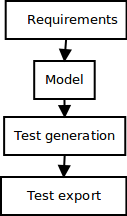
\includegraphics[scale=0.6]{img/conformiq_process.png}
\caption{MBT process in Conformiq}
\label{fig:conformiq_process}
\end{figure}

\begin{enumerate}
	\item First step is specifying requirements. Conformiq support a huge amount of industrial requirements modelling tool (eg.: IBM Rational, Rhapsody, Sparx Systems Enterprise, ArchitectHP Quality Center, IBM RequisitePro, DOORS), but it contains an own editor too. The defined requirements are traceable through the whole software testing process.
	\item Based on the requirements one has to create the model of the SUT. It can be done with the Conformiq Designer internal model editor using its QML language. The language consists three parts: system block diagrams, which describes the interface of the model (inbound and outbound ports); UML statecharts and Java like action language.
	\item After the modelling phase abstract test cases can be generated. The generation starts with transforming the model to an intermediate Lisp model, that is used during the symbolic execution, which generates the use cases. The user is able to see coverage statistics and a traceability matrix based on the generated test cases.
	\item Abstract test cases have to be exported with so called scripting backend which creates concrete test cases for the SUT.
\end{enumerate}

% subsection conformiq (end)

\subsection{Conclusion}
\label{sub:conclusion}

After investigating five widely used MBT tools, we can draw some consequences.

\begin{table}[htb]
\begin{center}
\begin{tabular}{|l|l|l|l|}
\hline
	\textbf{Name of the tool} & \textbf{Model} & \textbf{Intermediate model} & \textbf{TC generation method}\\\hline
	GraphWalker & UML & GraphML & search based, combinatorial, random\\\hline
	PyModel & FSM + Python & graph & search based\\\hline
	Conformiq & QML & Lisp (CQ$\lambda$) & symbolic execution\\\hline
	GOTCHA & EFSM & graph & BFS, DFS\\\hline
	ParTeG & UML + OCL & graph & DFS\\
\hline
\end{tabular}
\end{center}
\caption{\label{tab:toolssummary} Summary of examined MBT tools}
\end{table}

\begin{itemize}
	\item Creators of these tools either try to use an UML like model or FSM (EFSM). FSM models are low level representations of the SUT, so implementing search based algorithms and graph traversal algorithms are relatively easy. When tools using UML model with graph intermediate model, they can not support complex UML state chart elements, such as orthogonal regions.
	\item The intermediate model is just always some kind of graph representations, because the test case generation algorithms are the easiest to implement using graph models (search based test case generation, coverage criteria).
	\item Important thing to note, that the most successful tools use symbolic execution and it can handle the most complex models.
\end{itemize}

% subsection conclusion (end)

% section mbttools (end)

\newpage

\section{Implementation of test case generation algorithms}
\label{sec:implementation}

At the implementation phase I experimented with three algorithms. My goal was to implement graph traversal algorithms, which can be combined with an extended state machine. The extended state machine will have actions and guards, besides the events. These guards interpreted on the edges of the graph, and the actions are interpreted on nodes and on edges too. A sample state machine can be see on Figure~\ref{fig:statechartguard}.

\begin{figure}[htp]
\centering
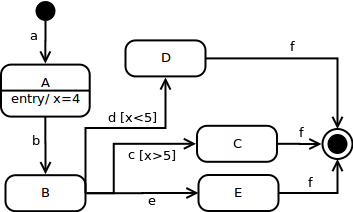
\includegraphics[scale=0.5]{img/guard1.png}
\caption{Example for state chart with guards and actions}
\label{fig:statechartguard}
\end{figure}

First I extended the previously studied Chinese Postman Problem (CPP) algorithm (Section~\ref{sec:intro}) with guards and actions. The effectiveness of this method for test case generation is not useful generally, because the CPP algorithm can be used exclusively with resettable softwares, which can back to their starting state. During the CPP graph traversal at every action, the Eulerization phase of the CPP algorithm has to be executed again. That's why this algorithm has a big computational overhead when combined with guards and actions.

After that I implemented breadth-first (BFS) and depth-first (DFS) algorithm combined with guards I saw the differences between the two algorithm. They can only used with state based coverage criterion, but it is easy to implement both algorithms. BFS generates a lot of short test cases, whilst DFS generates fewer, but very long test cases from a given state machine. The difference between the use cases can be see on Table~\ref{tab:bfsdfsresults} based on the given state machine Figure~\ref{fig:statechartguard}.

\begin{table}[htb]
\begin{center}
\begin{tabular}{l}
	\textbf{BFS}: \\
	a $\rightarrow$ b $\rightarrow$ d \\
	a $\rightarrow$ b $\rightarrow$ e \\
	a $\rightarrow$ b $\rightarrow$ d $\rightarrow$ f \\
	a $\rightarrow$ b $\rightarrow$ e $\rightarrow$ f \\\hline
	\textbf{DFS}: \\
	a $\rightarrow$ b $\rightarrow$ d $\rightarrow$ f \\
	a $\rightarrow$ b $\rightarrow$ e $\rightarrow$ f
\end{tabular}
\end{center}
\caption{\label{tab:bfsdfsresults} Generated test cases with BFS and DFS}
\end{table}

% section implementation (end)

\section{Summary and further development}
\label{sec:summary}

Previous semester I studied the MBT terminology, taxonomy and the general testing process. Based on these experiences this semester I extended my knowledge with test case generation methods and software representation models.

Three new industrial MBT tool have been examined concentrating on their model and the intermediate model that serves as a base for test case generation algorithms. Conclusion of the review can be utilised in later works.

Finally the work has been summarised implementing graph traversal algorithms, where the state machines are extended with guards and actions as well.

After deep understanding of MBT techniques and technologies, next semester it may be possible to start designing and developing a software which fills the need of a fully automated testing framework.

% section summary (end)

% Bibliography
\clearpage
\nocite{*}
\bibliographystyle{plain}
\bibliography{/home/chef/Egyetem/Onlab1/msc-thesis/doc/unicsovicsmilangyorgy_jzk2.bib}

\end{document}
